\documentclass[sigconf,nonacm]{acmart}

\usepackage{booktabs}
\usepackage{multirow}
\usepackage{enumitem}
\usepackage{amsmath}
\usepackage{array}
\usepackage{xspace}
\usepackage{hyperref}
\graphicspath{{../figures/evaluation/}}

% paper-specific
\newcommand\vldbdoi{XX.XX/XXX.XX}
\newcommand\vldbpages{XXX--XXX}
% issue-specific
\newcommand\vldbvolume{20}
\newcommand\vldbissue{1}
\newcommand\vldbyear{2027}
% should be fine as it is
\newcommand\vldbauthors{\authors}
\newcommand\vldbtitle{\shorttitle}
\newcommand\vldbavailabilityurl{https://github.com/M1zukiqwq/PVLDB2027-SAKI-OpenSource}
\newcommand\vldbpagestyle{plain}

\newcommand{\rocksdb}{RocksDB\xspace}
\newcommand{\sysname}{SAKI\xspace}
\newcommand{\ratecall}{\texttt{RateLimiter::\allowbreak SetBytesPerSecond()}\xspace}
\newcommand{\maxbgjobs}{\texttt{max\_\allowbreak background\_\allowbreak jobs}\xspace}
\newcommand{\staticbiased}{\texttt{static\_\allowbreak biased}\xspace}
\newcommand{\staticautotuned}{\texttt{static\_\allowbreak autotuned}\xspace}
\newcommand{\epochdrift}{\textsc{Epoch-Drift16}\xspace}
\newcommand{\runtimedrift}{\textsc{Runtime-Drift16}\xspace}
\newcommand{\valuefourk}{\textsc{Value-4K}\xspace}
\newcommand{\readthreex}{\textsc{Read-3x}\xspace}
\newcommand{\fastdrift}{\textsc{Fast-Drift}\xspace}
\newcommand{\tenantseight}{\textsc{Tenant-8}\xspace}
\emergencystretch=3em
\sloppy

\begin{document}
\raggedbottom

\title{SAKI: Shared Adaptive KV-Instance Control under a Fixed Compaction Budget}

\author{Qichu Tian}
\affiliation{%
  \institution{Xi'an Jiaotong University}
}
\email{mizukiqwq@stu.xjtu.edu.cn}

\author{Heng Chen}
\affiliation{%
  \institution{Xi'an Jiaotong University}
}
\email{hengchen@xjtu.edu.cn}

\author{Shipeng Zhao}
\affiliation{%
  \institution{Xi'an Jiaotong University}
}
\email{zhaoshipeng@stu.xjtu.edu.cn}

\author{Bo Wang}
\affiliation{%
  \institution{Xi'an Jiaotong University}
}
\email{Aroom@stu.xjtu.edu.cn}

\begin{abstract}
Multi-tenant deployments often co-locate many \rocksdb instances on one host.
Each tenant has an independent LSM pipeline, but flushes and compactions draw
from a shared background I/O and compaction budget. When write pressure drifts,
equal per-instance allocation can leave service stranded at quiet tenants while
tenants creating compaction debt suffer high write-tail latency. We frame this
as fixed-budget placement: moving the existing background budget toward tenants
where compaction pressure is forming.

SAKI is an external controller for this placement problem. In its conserved
rank-and-assign framework, the controller observes per-tenant demand and
pressure symptoms, ranks tenants without oracle labels or workload forecasts,
and reallocates per-tenant background budgets while preserving the aggregate
budget. A demand-observability model explains when demand-aware ranking keys
track bounded drift within one window and why pressure-only ranking can suffer
stale-debt lag. SAKI requires no changes to \rocksdb's compaction algorithm or
tenant application code. Across five
16-tenant epoch-level drift trials, SAKI reduces high-pressure write P99 by
11.7\%, raises high-pressure throughput by 38.1\%, and lowers compaction write
bytes by 21.0\% relative to equal static allocation, while keeping total
throughput roughly neutral. In a continuous embedded \rocksdb harness with
long-running tenants and runtime actuation through \ratecall, SAKI reduces
high-pressure write P99 by 27.0\%, reduces P999 by 47.1\%, raises
high-pressure throughput by 26.1\%, and lowers normalized bytes/write by
11.9\%. Stronger baselines, ranking replay, ranking-key perturbations, and
mechanism checks attribute these gains to online placement rather than extra
capacity, static skew, ranking-key fragility, or unrelated throttling. Public-trace
audits identify what future production traces must preserve for controller
validation. The results show that shared
compaction budgeting is a practical host-level control point for multi-tenant
\rocksdb deployments under fixed background budgets.
\end{abstract}


\maketitle

%%% do not modify the following VLDB block %%
%%% VLDB block start %%%
\pagestyle{\vldbpagestyle}
\begingroup\small\noindent\raggedright\textbf{PVLDB Reference Format:}\\
\vldbauthors. \vldbtitle. PVLDB, \vldbvolume(\vldbissue): \vldbpages, \vldbyear.\\
\href{https://doi.org/\vldbdoi}{doi:\vldbdoi}
\endgroup
\begingroup
\renewcommand\thefootnote{}\footnote{\noindent
This work is licensed under the Creative Commons BY-NC-ND 4.0 International License.
Visit \url{https://creativecommons.org/licenses/by-nc-nd/4.0/} to view a copy of this license.
For any use beyond those covered by this license, obtain permission by emailing
\href{mailto:info@vldb.org}{info@vldb.org}. Copyright is held by the owner/author(s).
Publication rights licensed to the VLDB Endowment. \\
\raggedright Proceedings of the VLDB Endowment, Vol. \vldbvolume, No. \vldbissue\ %
ISSN 2150-8097. \\
\href{https://doi.org/\vldbdoi}{doi:\vldbdoi} \\
}\addtocounter{footnote}{-1}\endgroup
%%% VLDB block end %%%

%%% do not modify the following VLDB block %%
%%% VLDB block start %%%
\ifdefempty{\vldbavailabilityurl}{}{
\vspace{.3cm}
\begingroup\small\noindent\raggedright\textbf{PVLDB Artifact Availability:}\\
The source code, data, and/or other artifacts have been made available at \url{\vldbavailabilityurl}.
\endgroup
}
%%% VLDB block end %%%

\section{Introduction}

Modern data-serving systems often place many storage-engine tenants on one
host. Each tenant may own a separate \rocksdb instance, data directory,
configuration, and foreground workload, yet their flushes and compactions draw
from the same finite background CPU and storage bandwidth. Per-instance controls are
useful, but they do not decide how a fixed host budget should be divided
across competing instances.

This placement decision becomes a performance problem when demand drifts. Equal
static allocation leaves capacity assigned to quiet tenants; frozen skew becomes
stale when the high-pressure set moves; and RocksDB's per-instance auto-tuned
rate limiter adapts within a configured ceiling but cannot move budget across
instances. The resulting compaction-debt mismatch appears as high write-tail
latency and lower completion rates for tenants currently creating debt.

We study the host-level placement decision directly. Under a fixed aggregate
background compaction/I/O budget, can an online controller use runtime
observations to reallocate per-tenant budgets across co-located \rocksdb
tenants, improving the tenants currently under write pressure without oracle
labels, workload forecasts, or extra host capacity? The question is
not whether more compaction capacity helps, but whether the same capacity can
be placed better than fixed fair sharing.

Several close directions leave this placement point open. General
multi-tenant storage controllers enforce lower-layer I/O shares or SLOs, while
recent LSM-oriented systems either change a single engine, move flush or
compaction into a disaggregated service or DPU path, or build isolation into a
different multi-tenant engine boundary~\cite{gulati2010mclock,
thereska2013ioflow,yu2024caaslsm,ding2025dflush,wang2026flexengine,
griggs2026deltafairsharing}. SAKI instead targets a common operational shape:
many separate, unmodified \rocksdb instances on one host, with only a conserved
background budget to place across them as demand drifts.

SAKI is an external controller for this placement problem. It observes each
tenant over a control window, ranks tenants using offered write demand and
compaction-pressure symptoms, and applies the next-window budget assignment
while conserving the aggregate budget. This conserved rank-and-assign framework
separates the placement invariant from the ranking key. Its key condition is
demand observability: when offered demand separates currently high-pressure
tenants from the rest, demand-aware ranking keys track bounded drift within
one control window, while pressure-only ranking can chase stale debt. SAKI sits
outside RocksDB; in the continuous harness, it changes runtime rate-limiter
budgets through \ratecall.

The evaluation follows an attribution chain. It first asks whether SAKI improves
the target tenants under the same aggregate budget, using both epoch-level and
continuous \rocksdb experiments. It then tests alternative explanations,
including static skew, tenant-local autotuning, stale-debt scoring, lower-layer
I/O weights, and foreground throttling. Finally, ranking-margin replay,
ranking-key perturbations, workload-matrix experiments, collateral measurements,
liveness checks, and public-trace audits define where the evidence applies.

In a 16-tenant epoch-level workload, five trials show that SAKI reduces
high-pressure write P99 by 11.7\%, raises high-pressure throughput by 38.1\%,
and lowers compaction write bytes by 21.0\% relative to equal static allocation,
with roughly neutral total throughput. In a continuous embedded \rocksdb harness
with runtime actuation, five trials show that SAKI reduces high-pressure write
P99 by 27.0\%, reduces P999 by 47.1\%, raises high-pressure throughput by
26.1\%, and lowers normalized bytes/write by 11.9\%. The tradeoff is visible:
lower-pressure tenants may absorb part of the cost, so SAKI is a targeted
reallocation policy.

The paper makes five contributions:
\begin{enumerate}[leftmargin=1.2em,itemsep=0pt,topsep=2pt]
\item It frames multi-tenant \rocksdb compaction as a fixed-budget host-level
reallocation problem, distinct from single-instance compaction-policy design.
\item It presents SAKI, a conserved rank-and-assign controller that sets
per-tenant runtime budgets from previous-window observations without oracle
labels, workload forecasts, or tenant application changes.
\item It identifies the demand-observability condition that lets a
demand-aware ranking key track bounded drift, and contrasts it with the
stale-debt lag of pressure-only ranking.
\item It provides epoch-level and continuous evidence that online reallocation
improves high-pressure write latency and throughput under bounded drift while
keeping total throughput close to static allocation.
\item It separates SAKI's effect from fixed skew, per-instance local autotuning,
ranking-key choice, workload variation, and lower-layer I/O control, while
making collateral costs and validation boundaries explicit.
\end{enumerate}

Together, these results show that shared host-level compaction budgeting is a
practical control point for multi-tenant \rocksdb write performance under
bounded drift.

\section{Background and Motivation}

SAKI targets co-located \rocksdb instances whose background work shares finite
host resources. RocksDB exposes useful local controls, but not the host-wide
placement decision: how that fixed service budget should be placed across
instances as tenants' write pressure changes at different times.

\subsection{LSM Background Work}

The log-structured merge-tree makes foreground writes inexpensive by buffering
updates and later merging them into on-disk components~\cite{oneil1996lsm}.
Compaction rewrites sorted files, removes obsolete entries, controls level
sizes, and bounds read cost. This design gives high write throughput but turns
recent foreground writes into future CPU and I/O demand. That deferred demand
becomes a host-level problem when several engines share one finite background
budget; surveys and recent microbenchmarks emphasize compaction, amplification,
and buffering as central LSM tradeoffs~\cite{luo2020lsmsurvey,
kaushik2024lsmbuffer}.

RocksDB exposes per-instance background jobs, rate limiters, statistics,
properties, and event listeners~\cite{rocksdb}. SAKI uses them as the
measurement and actuation surface for the host-level placement problem.

\subsection{From Tenant-Local State to Host-Level Debt}

We use \emph{compaction debt} as an operational term for deferred background
work and its foreground consequences. Pending compaction bytes, L0 files,
flush/compaction events, write-tail latency, and completion gaps are observable
but incomplete symptoms that help identify tenants currently creating deferred
maintenance.

The cross-tenant aspect is the key. Under a fixed aggregate budget, equal
allocation leaves capacity assigned to quiet tenants whenever only a subset is
write-heavy. Frozen skew helps only while the workload resembles the phase it was
tuned for. Section~\ref{sec:evaluation} tests this mismatch between where the
budget sits and where debt is being created.

Compaction service has delayed effects: too little service may surface later as
L0 pressure, flush backlog, write slowdown, or tail latency; too much service
for a quiet tenant consumes capacity that could reduce risk elsewhere. The
evaluation therefore reports high-pressure latency and throughput together with
total throughput and collateral impact on lower-pressure tenants.

\subsection{Why Existing Directions Do Not Settle the Question}

Prior LSM work changes single-engine policies or storage layout: Monkey,
Dostoevsky, WiscKey, PebblesDB, and SILK improve what an engine does given an
assigned service budget~\cite{dayan2017monkey,dayan2018dostoevsky,
lu2016wisckey,raju2017pebblesdb,balmau2019silk}. SAKI asks where a fixed host
budget should be placed across independent engines.

CaaS-LSM treats compaction as a service and DFlush offloads flush work to
DPUs~\cite{yu2024caaslsm,ding2025dflush}. SAKI shares the resource-management
view, but targets co-located RocksDB instances on one host, standard runtime
controls, and a conserved aggregate budget. The next section formalizes that
host-level allocation question.

\section{Problem Definition}

We study a host with tenants \(T=\{1,\ldots,N\}\). Each tenant is an
independently configured \rocksdb instance with its own memtables, WAL, SST
files, flush path, compaction path, and foreground workload. Tenants do not
share logical key spaces, but their background work draws from shared host
resources. Time is divided into control windows \(w=1,2,\ldots\). In each
window, the controller assigns tenant \(i\) a background budget \(b_i(w)\). The
unit of this budget is harness-dependent: epoch runs change rate limits and
background-job settings between epochs, while continuous runs keep tenants alive
and change the rate-limiter budget through \ratecall.

The aggregate budget is fixed. If \(B\) is the host budget, a valid assignment
must satisfy \(\sum_i b_i(w)=B\), subject to the discrete budget tiers exposed by
the implementation. Without this conservation rule, a controller could improve
high-pressure tenants simply by spending more host capacity.

The controller is online. At the start of window \(w\), it may use only
observations from windows up to \(w-1\). The observation vector \(x_i(w-1)\)
can include demand signals such as offered write demand and completed write
throughput; pressure symptoms such as completion gap, write-tail latency,
pending-compaction proxies, and L0 pressure; background-work signals such as
compaction bytes and flush/compaction events; read-side measurements; and the
prior assignment. It may not include the next high-pressure set, future phase
id, or evaluator-only tier labels. SAKI also does not observe a single
ground-truth scalar called compaction debt; it observes symptoms of deferred
work and foreground pressure.

The objective is targeted relief for tenants currently under high write
pressure, measured by write-tail latency and write throughput, while preserving
attribution to online reallocation under a fixed budget. Because reallocation is
a tradeoff, collateral effects must also be visible: the evaluation reports
mid- and low-pressure effects, total throughput, and liveness failures. Each
decision therefore chooses \(b_i(w)\) from implementable budget levels using
\(x_i(w-1)\), conserving \(B\) under delayed feedback.

Several constraints sharpen the scope. Policies cannot read workload labels or
future drift schedules. Continuous runs actuate only the runtime rate limiter,
rather than every RocksDB option. Assignments occur at window boundaries, so
very fast drift may outrun a previous-window controller. SAKI is therefore not a
new compaction algorithm, an in-engine global scheduler, or an oracle
classifier. The definition leaves the ranking rule open; the next section
instantiates this online fixed-budget problem with a conserved rank-and-assign
framework and a transparent demand-aware ranking key.

\section{SAKI Design}
\label{sec:saki-design}

\begin{figure*}[!t]
  \centering
  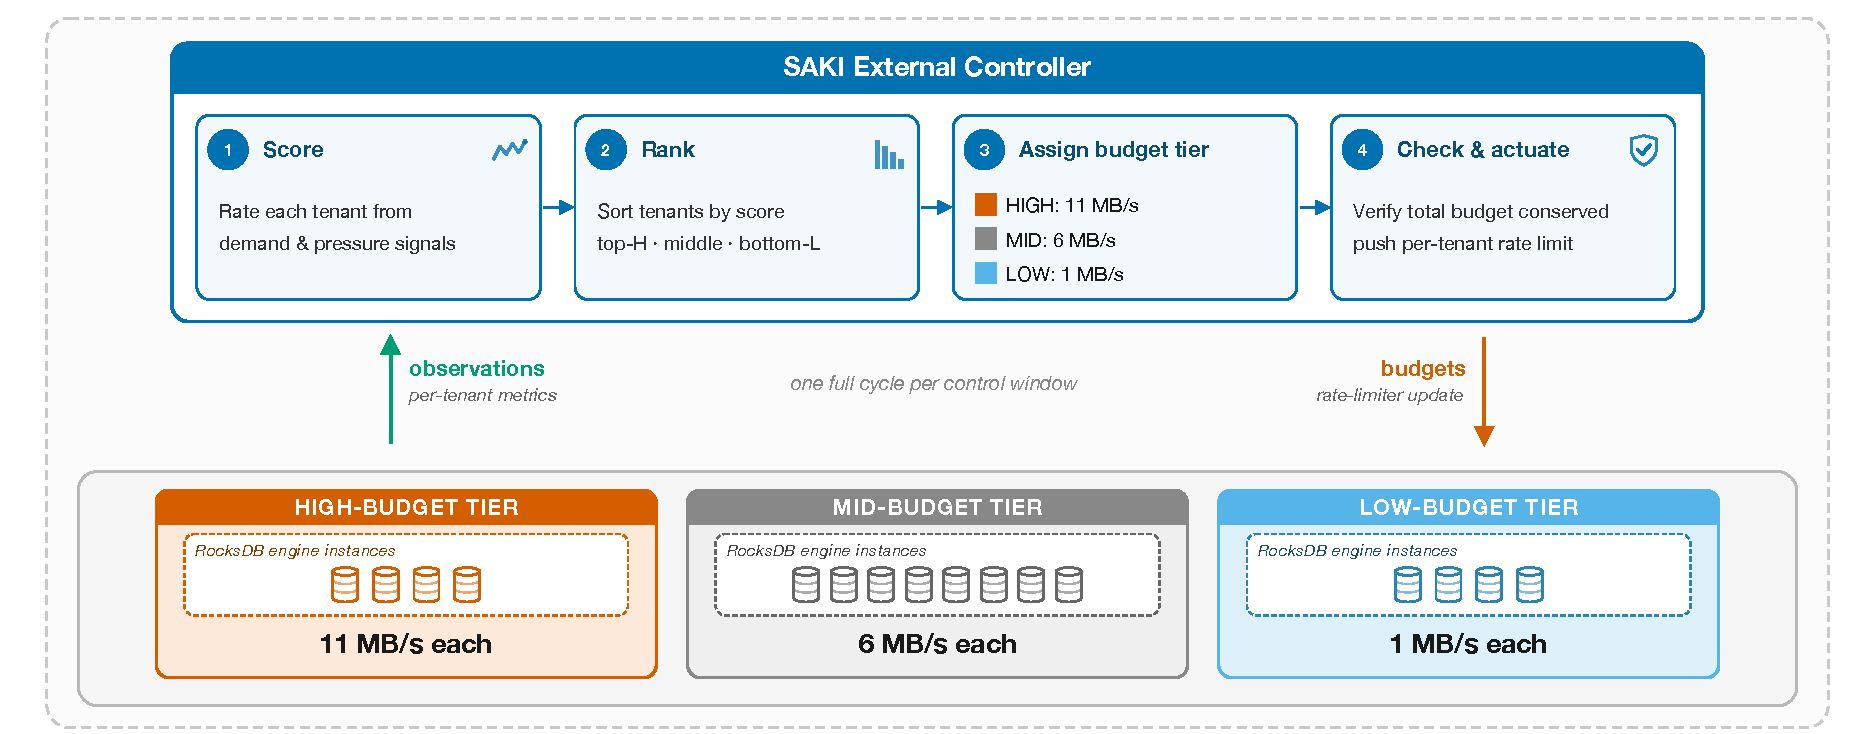
\includegraphics[width=0.95\textwidth]{fig1_saki_framework.pdf}
  \caption{SAKI conserved rank-and-assign loop. Each window, the external
  controller scores tenants from previous-window demand and pressure signals,
  ranks them, assigns high/mid/low budget tiers, checks that the aggregate
  host budget is preserved, and pushes runtime rate-limit updates. The shown
  $4{:}8{:}4$ split at $11{:}6{:}1$\,MB/s is the main continuous setting.}
  \Description{Architecture diagram of SAKI. An external controller box at the
  top contains four pipeline steps: Score (rate each tenant from demand and
  pressure signals), Rank (sort by score), Assign budget tier (HIGH/MID/LOW
  at 11/6/1 MB/s), and Check and actuate (verify total budget conserved, push
  per-tenant rate limit). A closed loop runs every control window:
  observations flow up from the tenant pool to the controller, and budget
  updates flow down via the runtime rate limiter. The tenant pool at the
  bottom is one outer frame containing three tier cards, each with a labeled
  dashed sub-frame holding mini cylindrical RocksDB engine icons: four engines
  in the HIGH-budget tier, eight in the MID-budget tier, and four in the
  LOW-budget tier.}
  \label{fig:saki-framework}
\end{figure*}

SAKI is a host-level closed-loop controller that implements a conserved
rank-and-assign framework, sketched in Figure~\ref{fig:saki-framework}. The
framework is the method contribution: it preserves a fixed-budget invariant
and assignment template while allowing different observable score instances
to rank tenants. SAKI sits outside RocksDB, observes each tenant over window
\(w\), assigns budget tiers for window \(w+1\), and validates that the
aggregate budget is unchanged. The one-window delay is intentional: signals
from window \(w\) must remain informative for window \(w+1\).

\subsection{Conserved Rank-and-Assign Framework}

The framework decouples a budget-conserving assignment template from the score
instance used to rank tenants. The control loop, illustrated by the four
pipeline steps in Figure~\ref{fig:saki-framework}, is intentionally compact:
\[
\begin{array}{ll}
\textbf{Input:} & \{x_i(w)\}_{i=1}^{N},\; B,\; b_H,b_M,b_L,\; H,L \\
\textbf{Score:} & s_i(w) \leftarrow \mathrm{score}(x_i(w)) \\
\textbf{Rank:} & \text{sort tenants by descending } s_i(w) \\
\textbf{Assign:} & \text{top }H\rightarrow b_H,\; \text{bottom }L\rightarrow b_L,\;
\text{others}\rightarrow b_M \\
\textbf{Check:} & \sum_i b_i(w+1)=B \\
\textbf{Actuate:} & \text{apply } b_i(w+1) \text{ for the next window.}
\end{array}
\]
The tiered assignment makes the policy auditable. We distinguish
\emph{high-pressure} tenants, which the workload currently stresses, from
\emph{high-budget} tenants, which SAKI assigns to \(b_H\). A tier configuration
is budget-conserving when \(H(b_H-b_M)=L(b_M-b_L)\); the continuous main
setting uses \(4(11-6)=4(6-1)\), yielding the same 96\,MB/s aggregate budget as
sixteen all-mid tenants. Other tier counts or continuous allocations can use
the same rule; we fix auditable tierings to isolate the placement mechanism
within each experiment family.

The score instance instantiates the framework; it is not the framework itself.
This separation lets the paper make a framework claim and then test a small
family of auditable instances under the same conserved assignment rule. The
reference instance below is intentionally simple so the evaluation attributes
gains to online placement under conservation, not to an opaque learner or extra
capacity.

\subsection{Observations and Labels}

The observation vector is tenant-local, but the decision is host-wide. In the
continuous harness, \(x_i(w)\) includes offered write/read rates, completed
operations, write latency percentiles, compaction and flush bytes from an event
listener, estimated pending compaction bytes, L0 files, memtable bytes,
delayed-write rate, write-stop status, and the current assignment. These are
runtime measurements rather than workload labels.

The experiment generator retains each tenant's synthetic workload tier so the
evaluation can compute high-pressure benefit and high-set overlap. The
controller does not read that tier, a future phase identifier, or the next
high-pressure set. Offered write demand is an observed admission-side signal
from the previous window, rather than a prediction.

\subsection{Reference Score Instance and Family}

SAKI supports several score instances for ablation studies. The main continuous
policy uses a demand-aware reference instance. Let \(D_i\) be offered write
QPS, \(C_i\) completed write QPS, \(G_i=\max(0,D_i-C_i)\) the completion gap,
\(B_i\) the compaction output in MB, \(P_i\) pending compaction bytes in MB,
and \(L_i\) the number of L0 files capped at 6. The bounded tail term is
\[
T_i=\min(\mathrm{P99}_i/1000,80)+\min(\mathrm{P999}_i/5000,40),
\]
where latency is measured in microseconds. In demand mode, SAKI scores tenant
\(i\) as
\[
s_i =
6.00 D_i/1000
+0.60 G_i/1000
+0.05 T_i
+0.02 B_i
+0.02 P_i
+0.30 L_i .
\]
The coefficients reflect a design choice, not a universal optimum. Offered
write demand anchors active high-pressure tenants, while bounded residual
terms---completion gap, tail latency, compaction output, pending bytes, and L0
pressure---refine near-boundary tenants. This division targets two failures:
pressure-only scores can chase stale debt after demand moves, while demand-only
scores lack a maintenance signal for tenants that have just left a high-demand
phase. Residuals should not overturn a clearly separated demand signal, but
can stabilize rankings when margins are small. The evaluation tests this with
offline decision replay and online coefficient perturbations; in the main
continuous workload, replaying all 35 post-warmup decisions shows that the
demand term alone reproduces the full reference score's top-four assignment.

The score is fixed and auditable, but SAKI remains online: observations,
ranking, and assignment are recomputed every window. Keeping the rule fixed
separates the placement question from learning coefficients under delayed,
partially counterfactual feedback. The relevant design space is a family of
demand-aware instances whose primary term is offered write demand and whose
secondary pressure terms are bounded refinements. Section~\ref{sec:evaluation}
therefore tests demand-only replay, online anchor-scaled, residual-scaled, and
anchor-only instances, along with pressure-only negative controls, under the
same rank-and-assign template. This design yields two falsifiable predictions:
demand-aware instances should track moving pressure with high overlap and low
lag, while pressure-only instances should expose stale-debt lag. The
coefficients are not portable constants; deployments could add normalization or
policy layers while preserving budget conservation and demand observability.

The epoch harness uses a coarser, pressure-oriented score because each epoch
exposes clearer symptoms. The continuous harness is stricter: decisions are made
every short window while tenants stay active. Demand mode is the main
continuous policy; pressure and hybrid modes serve as ablations.

\subsection{Actuation and Stability}

The actuation path matches the harness. Epoch-level runs can change
background-job and rate-limit settings between epochs. Continuous runs keep
each tenant active and adjust only the runtime rate-limiter budget; \maxbgjobs
remains fixed at process launch. Section~\ref{sec:implementation} gives the
specific runtime API.

SAKI's framework-level stability rests on budget conservation, bounded score
terms, tiered assignment, a low-tier floor, and one-window updates. We evaluate
this envelope through high-set overlap, adaptation lag, total throughput,
bytes/write, and tier-level collateral effects. Production deployments could
add hysteresis, cooldowns, minimum-dwell rules, or SLO-weighted floors.
Per window, the controller aggregates \(N\) tenant observations, sorts tenants
by score, validates the conserved budget, and issues \(N\) budget updates. The
control-plane work is \(O(N\log N)\) and stays outside the foreground write
path. The paper does not include an overhead-scaling sweep at larger tenant
counts.

\subsection{Analytical Motivation}
\label{sec:analysis}

The design choices in the preceding subsections are motivated by a simple
analytical model. The model is not an optimizer for the coefficients; instead,
it isolates the tracking condition that the score family must satisfy and
explains the experimental divergence between demand-mode and pressure-mode
controllers reported in Section~\ref{sec:evaluation}.

\emph{Model.}
Let tenant \(i\) have offered write demand \(d_i(w)\), completed write rate
\(c_i(b)\) under budget \(b\), and normalized compaction debt \(q_i(w)\) in
equivalent writes. Budget tiers satisfy \(b_H>b_M>b_L\) with conservation
\(H b_H+(N-H-L)b_M+L b_L=B\). Backlog evolves as
\[
q_i(w+1)=\max\!\bigl(0,\; q_i(w)+T\,(d_i(w)-c_i(b_i(w)))\bigr),
\]
where \(T\) is the window length. We call tenant \(i\) \emph{high-pressure}
when \(d_i(w)\) exceeds the service rate achievable under \(b_M\); the deficit
under \(b_L\) is larger still.

\emph{Why static allocation can fail.}
Under equal allocation \(b_i=B/N\), if a high-pressure tenant satisfies
\(d_i>c_i(B/N)\), then \(q_i\) grows without bound until a write stall or
SLO violation occurs. This is the baseline problem: equal sharing allocates the
fixed budget without regard to which tenants are currently creating debt.

\emph{Proposition 1 (demand-aware one-window tracking).}
Consider a score instance in the rank-and-assign framework whose ordering can
be written as \(s_i=\alpha D_i(w)+\rho_i(w)\), where \(D_i(w)\) is the
observed offered demand and the residual term \(\rho_i(w)\) is computed from
bounded pressure and maintenance signals. Suppose the high-pressure set to be
served has at most \(H\) tenants and remains active into the next control
window. If, in window \(w\), every such tenant has offered demand at least
\(\Delta\) above every non-high tenant and
\[
\alpha\Delta > \max_{i,j}|\rho_i(w)-\rho_j(w)|,
\]
then the framework places those tenants in the high-budget tier in window
\(w+1\).

The proof is immediate from the ordering condition: for any high-pressure
tenant \(i\) and non-high tenant \(j\), \(s_i-s_j>0\), so the top-\(H\) rank
contains the high-pressure set. The one-window delay is unavoidable because the
controller only observes \(D_i(w)\) after window \(w\) completes. The condition
is sufficient, not universal: in the continuous main trials, offline replay
shows that the demand term alone produces the same top-four assignment as the
reference score in all 35 post-warmup decisions.

\emph{Proposition 2 (stale-debt lag for pressure-only ranking).}
Consider a monotone pressure-only instance that ranks tenants by backlog or
maintenance signals but does not observe offered demand. Immediately after a
workload drift, the instance cannot distinguish an exiting tenant with
historical debt from an entering tenant whose current demand is forming fresh
debt. If the exiting tenant starts the post-drift period with residual pressure
equivalent to \(q\) writes above the entrant, and the extra drain rate gained
by removing its high-budget slot is at most \(\Delta c=c(b_M)-c(b_L)\), then
the stale high-budget assignment can persist for
\(\Omega(q/(T\Delta c))\) windows under a monotone backlog-priority rule.

This is not a convergence theorem for all controllers; it is a structural
ambiguity in the pressure-only family. It predicts the measured divergence
between score instances: demand mode tracks with overlap \(3.00/4\) and zero
max lag, while pressure-only mode has overlap \(1.86/4\) and max lag 5
windows. The coefficients remain a deployment choice, but the
demand-observability condition is the mechanism that separates tracking from
stale-debt chasing.

\section{Implementation}
\label{sec:implementation}

SAKI is implemented as an external Python controller plus two experiment
harnesses around unmodified \rocksdb instances. The implementation separates
the paper's two control questions and realizes the conserved rank-and-assign
framework from Section~\ref{sec:saki-design}. The epoch harness asks whether a
fixed budget can be placed better between workload phases; the continuous
harness asks whether the same placement loop can actuate a live RocksDB rate
limiter while tenants keep running. In both paths, the controller chooses high,
mid, and low budget assignments, the harness applies them through ordinary
RocksDB-facing APIs, and the measurement path records per-tenant behavior at
the same granularity used by the controller.

\subsection{Epoch Harness}

The epoch-level path uses \texttt{db\_bench} as the tenant process. A trial
creates one database directory per tenant, runs a prefill phase, and then
executes a sequence of workload epochs. Each epoch assigns tenants to high,
mid, and low demand tiers, launches one \texttt{db\_bench} process per tenant,
parses the logs, and uses the resulting observations for the next epoch's
allocation decision. Because every epoch is a fresh invocation, this harness
can vary both \texttt{max\_background\_jobs} and
\texttt{rate\_limiter\_bytes\_per\_sec} at epoch boundaries. The driver checks
that the resulting job and rate-limit settings match the static fair-share
budget before launch.

The parser extracts per-tenant runtime, exit status, operation rate, latency
histograms where available, compaction read/write bytes, flush bytes, keys and
bytes written, and compaction CPU time. It stores these rows with the epoch,
workload tier, assigned budget tier, background-job count, rate limit, and
workload parameters. This path gives clean mechanism evidence for budget
placement under drift because all policies run comparable foreground work under
the same aggregate budget. It does not by itself prove in-process runtime
control; that is the role of the continuous harness.

\subsection{Continuous Harness}

The continuous path is a custom C++ embedded RocksDB harness. Each tenant is a
long-running process linked against RocksDB. The Python driver writes one
control file per tenant, advances through fixed-length windows, computes the
current workload tier and policy assignment, validates the aggregate byte
budget, and atomically updates the control file. Tenant processes keep running
while their offered write/read rates, hot-key range, reported workload tier,
assigned budget tier, and byte budget are refreshed. Before each refresh the
driver checks that the next assignment preserves the aggregate byte budget.
Control files are written atomically, and a tenant keeps using its last
installed budget until it observes a newer value. Thus a missed or delayed
update does not create extra host budget in the harness; a production
controller would additionally fall back to all-mid allocation when tenant
inventory or metrics are incomplete.

Runtime actuation uses RocksDB's rate limiter. At startup, each tenant creates
a \texttt{NewGenericRateLimiter} with the initial budget and installs it before
opening the database. During the run, a control thread rereads the budget and
calls \ratecall on the same rate-limiter object. This is the main continuous
actuation path. Background-job count is a launch-time option and remains fixed
for the tenant process. Diagnostic userspace throttling exists in the harness
but is not the mechanism used for the reported continuous result.

The rate limiter is a RocksDB-facing background-I/O control rather than an
application-level admission throttle. In the reported setup it is installed as
the database rate limiter and therefore shapes the I/O issued by flush and
compaction work that uses RocksDB's rate-limited paths. SAKI does not directly
sleep foreground write calls or read calls. Foreground write latency changes
indirectly because background service changes the accumulation and draining of
LSM maintenance work. This distinction makes the continuous result a
maintenance-placement result rather than a foreground-throttling result:
SAKI changes the maintenance budget available to each tenant, not the offered
foreground workload. In the five main continuous trials, rate-limiter,
compaction, and flush byte deltas are larger in high-budget windows than in
low-budget windows. As an internal-validity check on this actuation path, we
also ran a homogeneous four-tenant static microstudy that sweeps the per-tenant
limiter budget \(B \in \{1,3,6,11\}\)\,MB/s with three seeds per point.
Dropping the first window, measured rate-limiter traffic is monotone in \(B\):
1.00, 2.96, 5.70, and 7.28\,MB/s. Compact-plus-flush output moves with the
limiter (coverage ratio 0.99--1.02); the 11\,MB/s point saturates at about
7.3\,MB/s because this workload cannot generate more maintenance I/O. A
two-seed no-rate-limiter sanity run reports zero limiter bytes while
background maintenance continues near 8\,MB/s. The microstudy shows that the
continuous knob controls background-maintenance I/O rather than foreground
throttling.

The embedded harness records per-window write and read operation counts,
throughput, and latency percentiles. A custom \texttt{EventListener} accumulates
compaction input/output bytes, compaction CPU time, compaction count, flush
bytes, and flush count. At window boundaries the harness emits deltas, together
with RocksDB properties such as pending compaction bytes, L0 files, memtable
bytes, delayed-write rate, and write-stop status. These measurements feed both
the online score and the post-run analysis.

\subsection{Analysis}

The analysis scripts consume JSON payloads produced by the drivers. For
continuous runs, the analyzer merges tenant metrics, allocation history,
process exit codes, commands, run parameters, and summary counters. It computes
write P99/P999 and throughput for high-pressure tenants, total throughput,
compaction output bytes, bytes/write, high-set overlap, adaptation lag, and
failed-tenant counts. The same pipeline emits the paper-table summaries and the
time-series data used for the evaluation figures. This keeps the manuscript
numbers tied to generated artifacts rather than manual transcription.

\section{Experimental Methodology}

The experiments are organized around the fixed-budget placement claim. The
first layer asks whether moving a host-level background budget toward tenants
currently carrying write pressure improves their write path without extra
capacity. The second layer narrows the mechanism: runtime actuation tests
deployable control, stronger baselines test fixed skew and local autotuning,
score instances test the adaptation signal, ranking replay and score-family
perturbations test robustness, cgroups test a lower-layer control point, and
the rate-limiter coverage microstudy checks the maintenance-I/O knob. The third
layer reports workload coverage, tier-wise collateral cost, liveness, and trace
qualification boundaries. Budget conservation is enforced within each
experiment family. The epoch-level and public-trace qualification runs use an
11/7/3\,MB/s, 112\,MB/s contract; the continuous runtime family uses an
11/6/1\,MB/s, 96\,MB/s contract. These numbers differ because the harnesses
expose different actuation surfaces, but every SAKI comparison holds the
relevant family budget fixed against its baselines.

\subsection{Workloads}

The epoch-level anchor is \epochdrift. It uses 16 co-located tenants, three
demand tiers, eight epochs, and gradual movement of a four-tenant
high-pressure set. Tenants are prefilled before the measured epochs.

The continuous anchor is \runtimedrift. It also uses 16 tenants and three
tiers, but runs tenants as long-lived embedded RocksDB processes for eight
20-second windows. The high-pressure set moves by one tenant per window, so the
experiment tests online adaptation at a rate the controller can plausibly
follow. The continuous anchor uses 11/6/1\,MB/s high/mid/low budgets with a
4/8/4 split, preserving a 96\,MB/s aggregate against an all-mid static
baseline. A window-length sensitivity bracket repeats the same anchor at 10,
20, and 40 seconds for three static/online seed pairs per point, holding the
160-second duration and all per-tenant budgets fixed. A score-family
robustness ablation perturbs the demand-mode instance along anchor weight and a
uniform residual scale ($\times 0.5$, $\times 2$, and $\times 0$ meaning
anchor-only), with three seeds per row paired with paper-static a/b/c; results
appear in Section~\ref{sec:evaluation}. We also replay all five continuous main
online traces offline to measure the ranking margin and the top-\(H\)
invariance of nearby score instances without launching additional RocksDB
runs. A separate 360-second longer-run is a sanity check for obvious
instability.

We also run a local sensitivity sweep around \epochdrift, changing drift
speed (\texttt{epochs\_per\_stage}=3 and 1, versus 2) and high write pressure
(70k and 130k writes/s, versus 100k). Each new point starts with two
\texttt{static}/SAKI screening trials; stress-side variants are promoted to
five trials if a pre-committed rule holds (high P99 improves by at least 2\%,
high throughput by at least 5\%, overlap $\ge$ 2.5/4, static does not hit
capacity-boundary).

Around \runtimedrift we run a controlled workload matrix that perturbs one
axis at a time: \valuefourk uses 4\,KB values, \readthreex triples per-tier
point-read QPS, \fastdrift moves the high-pressure set at 1.5 tenants per
window, and \tenantseight uses a smaller 8-tenant cluster with two
high-pressure tenants. Per-tenant budgets are preserved so the same-budget
contract holds; for \tenantseight the aggregate scales linearly. The matrix
uses the paper SAKI policy without changing the score instance. Every variant is
promoted from a two-trial screen to five trials unless either policy has a
failed tenant, and the overlap threshold is rescaled to each variant's
high-pressure tenant count.
The 20-second window, tier budgets, and 4/8/4 split are mechanism-isolation
settings, not portable constants. The 4/8/4 split is chosen because the
high-budget tier's surplus exactly matches the low-budget tier's savings,
preserving the same aggregate budget within each experiment family;
Section~\ref{sec:saki-design} states the general conservation rule.
\fastdrift and \tenantseight are local sensitivity, not a parameter search.

\subsection{Policies}

\texttt{static} is the main fair baseline: every tenant receives the same share
of the aggregate background budget for that experiment family. SAKI is the
online policy: it assigns high, mid, and low tiers from previous-interval
observations while preserving that aggregate budget. The main continuous SAKI
policy uses the demand-aware reference score instance.

\staticbiased is a frozen-skew baseline for the epoch workload. It uses the
same high/mid/low budget tiers, but freezes the initial-stage assignment for
all later epochs. It models an operator who pre-tunes a reasonable non-equal
allocation and then does not adapt as the high-pressure set drifts.

\staticautotuned is the strict same-budget built-in \rocksdb baseline. It uses
exactly the same per-tenant ceilings as \texttt{static}. In the epoch
configuration this is two background jobs and 7\,MB/s per tenant, for a 32-job
and 112\,MB/s aggregate budget across 16 tenants. Each tenant enables
\texttt{--rate\_limiter\_auto\_tuned=1}, so adaptation stays local to that
RocksDB instance and remains within the configured per-instance range. This
baseline asks whether per-instance local rate adaptation can replace the outer
host-level placement decision; we keep the ceilings identical to \texttt{static}.
For the sensitivity sweep, \staticautotuned is added only to the promoted
higher-pressure point.

\texttt{oracle\_tiered} is a diagnostic reference using true tier information.
\texttt{unlimited} is a capacity reference, not a same-budget competitor.

\subsection{Platform}
\label{sec:platform}

All experiments run on a single Linux machine with 80 logical cores (Ubuntu,
kernel 6.17). Storage is a local SSD. Each RocksDB tenant writes to its own
data directory on the same device. The epoch-level harness uses \texttt{db\_bench}
8.9.1 from unmodified Ubuntu \texttt{.deb} archives; the continuous harness
links against the same RocksDB version. No other major I/O-intensive processes
run during measured trials.

\subsection{Metrics and Aggregation}

Primary metrics are write P99/P999 latency and write throughput for
high-pressure tenants, the foreground symptoms SAKI is meant to improve by
moving background service. Total throughput shows whether the host collapses
aggregate work under the fixed budget. Tier-wise latency and throughput expose
the redistribution cost that a targeted policy can impose on lower-pressure
tenants. The continuous rate limiter is background-I/O control: it shapes
RocksDB flush/compaction I/O, so foreground changes reflect maintenance
placement rather than direct sleeps on application reads or writes.

Epoch-level efficiency reports compaction write bytes. In continuous runs SAKI
changes foreground completion, so the main compaction efficiency metric is
normalized bytes/write; absolute compaction bytes are reported but not the main
efficiency claim. Epoch runs execute comparable foreground work per trial, so
absolute background bytes are directly interpretable; continuous runs may
complete more foreground writes under SAKI and need per-write normalization.

Adaptation is measured by high-set overlap (high-pressure tenants assigned the
high-budget tier after warmup) and adaptation lag in control windows. Ranking
robustness is measured by replaying the previous-window observations that fed
each online decision and comparing the resulting top-\(H\) set across score
instances using exact-match count and Jaccard similarity. Liveness is measured
by failed tenant processes. The main epoch and continuous results aggregate
five independent trials. Percent changes are computed relative to static within
each trial before aggregation. The paper reports mean, range, standard
deviation, and confidence intervals. Sensitivity rows with two trials report a
mean and range; five-trial rows report 95\% CI half-widths. Raw and summarized
artifacts are recorded under \texttt{remote-results/}, and figures use real
result files from the figure data manifest.

\subsection{Scope}

The methodology supports a constrained claim: fixed-budget online reallocation
in two controlled RocksDB drift regimes. The built-in local rate-limiter
baseline is covered under the same aggregate budget because it tests whether
tenant-local adaptation can replace the host-level rank-and-assign loop.
OS/cgroup I/O controls are included for a different reason: they can enforce
weights or throttles below RocksDB, but they do not observe LSM debt signals or
decide which engine should receive compaction service. We include a 5-trial
aligned cgroup-v2 baseline at the same scale as the epoch main result (16
tenants, 8 epochs, 240k keys/tenant, 100k writes/high tier) as supplemental
mechanism evidence, not as a repeated main baseline. The controller inside the
cgroup harness uses a simplified pressure score for cross-mechanism comparison;
it is not the main SAKI controller used in the primary RocksDB experiments.

\section{Evaluation}
\label{sec:evaluation}

The evaluation follows the paper's fixed-budget claim through three questions.
First, within each harness's conserved budget contract, can RocksDB background
service do more useful work when placed on tenants currently creating
compaction debt? Second, is the effect online host-level placement rather than
extra capacity, static skew, local autotuning, a stale backlog signal, or a
lower-layer throttle? Third, what workload coverage, collateral cost, and
trace-qualification boundary remain after the mechanism is established?
Unless stated otherwise, percentages are online SAKI versus equal static
allocation; negative latency or bytes/write values are improvements, and
positive throughput values are improvements. In metric labels, ``High''
refers to the workload's high-pressure tenants; high-set overlap measures how
often those tenants receive SAKI's high-budget assignment. All reported
RocksDB and cgroup runs completed with zero failed tenants.

\subsection{Fixed-Budget Placement Improves High-Pressure Tenants}

The epoch-level harness isolates placement by changing RocksDB settings only
between epochs. Across five repeated 16-tenant drift trials, SAKI reduces
high-pressure write P99 by 11.7\%, raises high-pressure throughput by
38.1\%, and reduces compaction write bytes by 21.0\%
(Table~\ref{tab:evaluation-epoch-main}). Total throughput remains roughly
neutral: the mean is -1.7\%, and its CI crosses zero. All five trials improve
high-pressure write P99, high-pressure throughput, and compaction bytes; mean
high-set overlap is 3.14/4, so the policy places high budget near the moving
high-pressure set without using oracle labels.

\begin{table}[!t]
  \centering
  \caption{Epoch-level main result, \epochdrift (online vs.\ static).}
  \label{tab:evaluation-epoch-main}
  \small
  \begin{tabular}{lccc}
    \toprule
    Metric & Mean & Range & 95\% CI \\
    \midrule
    High write P99 & -11.7\% & [-17.2,-6.2] & [-18.0,-5.5] \\
    High throughput & +38.1\% & [+34.2,+42.1] & [+34.4,+41.7] \\
    Total throughput & -1.7\% & [-4.7,+2.1] & [-4.9,+1.4] \\
    Compact bytes & -21.0\% & [-24.3,-18.4] & [-23.6,-18.4] \\
    Mean high overlap & 3.14/4 & [3.14,3.14] & -- \\
    \bottomrule
  \end{tabular}
\end{table}

The continuous harness tests the stricter deployment boundary: tenants remain
alive, workload phases drift every 20 seconds, and SAKI changes only the
runtime rate-limiter budget through \ratecall. Table~\ref{tab:evaluation-continuous-main}
and Figure~\ref{fig:continuous-runtime} summarize five
\runtimedrift trials. SAKI reduces high-pressure write P99 by
27.0\%, P999 by 47.1\%, and raises high-pressure write throughput by 26.1\%.
Because SAKI completes more foreground writes, normalized bytes/write is the
main continuous efficiency metric; it falls by 11.9\%, while absolute compact
bytes change only -1.9\%. The continuous result shows the placement effect is
not an epoch artifact: the same conserved-budget loop works while tenants stay
alive and only the RocksDB rate-limiter budget changes.

\begin{table}[!t]
  \centering
  \caption{Continuous main result, \runtimedrift (five trials, online vs.\
  static).  CI half-widths in pp.}
  \label{tab:evaluation-continuous-main}
  \small
  \setlength{\tabcolsep}{3.2pt}
  \begin{tabular}{lcccc}
    \toprule
    Metric & Mean & Min & Max & 95\% CI \\
    \midrule
    High write P99 & -27.0\% & -39.2\% & -12.0\% & $\pm$12.5pp \\
    High write P999 & -47.1\% & -54.0\% & -39.3\% & $\pm$8.8pp \\
    High write throughput & +26.1\% & +21.5\% & +28.2\% & $\pm$3.5pp \\
    Total throughput & +4.3\% & +1.3\% & +6.8\% & $\pm$3.2pp \\
    Compact bytes & -1.9\% & -5.8\% & -0.1\% & $\pm$2.9pp \\
    Bytes/write & -11.9\% & -13.5\% & -9.1\% & $\pm$2.3pp \\
    Mean high overlap & 3.00/4 & 3.00 & 3.00 & -- \\
    \bottomrule
  \end{tabular}
\end{table}

\begin{figure}[t]
  \centering
  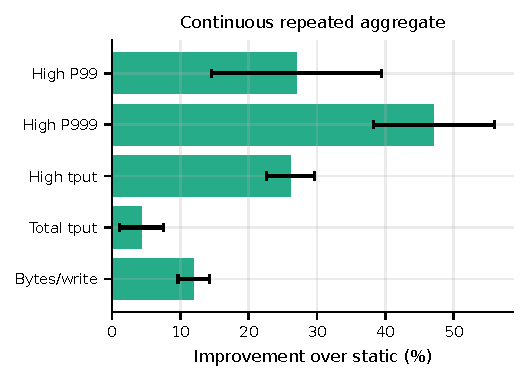
\includegraphics[width=\columnwidth]{fig3_continuous_summary.pdf}
  \caption{Continuous repeated aggregate. Each bar is normalized so positive
  means improvement over equal static; error bars show 95\% CI half-widths.}
  \Description{Horizontal bar chart of continuous-run improvements over
  static: high-pressure write P99, P999, high-pressure throughput, total
  throughput, and
  bytes/write.}
  \label{fig:continuous-runtime}
\end{figure}

\subsection{Mechanism Checks and Alternative Controls}
\label{sec:cgroup-baseline}

A fixed-budget improvement could be an artifact of a weak baseline, a stale
or fragile score instance, a non-maintenance throttle, or a lower-layer control
that already does the work. The checks in this subsection separate those
possibilities from online cross-tenant placement.

\begin{table*}[!t]
  \centering
  \caption{Mechanism checks against stronger same-budget baselines.  Rows use
  the comparison named at left, not all rows relative to static.}
  \label{tab:evaluation-stronger-baselines}
  \small
  \setlength{\tabcolsep}{4.4pt}
  \begin{tabular}{lcccccl}
    \toprule
    Comparison & High P99 & High tput & Total tput & Compact bytes & Mid tput & Overlap \\
    \midrule
    SAKI vs static & -11.7\% & +38.1\% & -1.7\% & -21.0\% & -9.1\% & 3.14/4 \\
    static\_biased vs static & -6.1\% & +17.4\% & -4.2\% & -9.9\% & -10.0\% & 1.14/4 \\
    static\_autotuned vs static & +28.8\% & -19.7\% & -1.8\% & -0.2\% & -17.3\% & 0.00/4 \\
    SAKI vs static\_biased & -6.0\% & +17.7\% & +2.8\% & -12.3\% & +1.1\% & 3.14 vs 1.14 \\
    SAKI vs static\_autotuned & -31.5\% & +71.9\% & +0.3\% & -20.8\% & +10.0\% & 3.14 vs 0.00 \\
    \bottomrule
  \end{tabular}
\end{table*}

Could equal static allocation simply be too weak a baseline?
Table~\ref{tab:evaluation-stronger-baselines} compares against a frozen skewed
allocation that helps the initial phase. Once the high-pressure set drifts,
however, its overlap falls to 1.14/4; SAKI recovers high-pressure throughput
(+17.7\% versus frozen skew), reduces compact bytes (-12.3\%), and restores
overlap to 3.14/4.

RocksDB's local auto-tuned rate limiter addresses a different problem: each
instance adapts within its configured ceiling, but unused budget is not moved
across tenants. Under the same per-tenant ceilings, \staticautotuned worsens
high-pressure P99 by 28.8\%, lowers high-pressure throughput by 19.7\%, and
has 0.00/4 high-set overlap. The same conclusion holds on the promoted
higher-pressure sensitivity point: \staticautotuned again worsens
high-pressure P99 by 29.5\% and lowers high-pressure throughput by 16.2\%
relative to static, while SAKI improves over it by 32.7\% on P99 and 59.9\%
on throughput.

A score instance that merely chases stale debt would lag the moving
high-pressure set. Pressure mode is a backlog-only online instance: it improves
high-pressure P99 ($-14.1\%$) but lags drift (overlap 1.86/4, max lag
5 windows). Demand mode adds the previous-window offered write signal, raises
overlap to 3.00/4, eliminates the 5-window lag, and raises high-pressure
throughput from +9.8\% to +26.1\%. Hybrid mode gives larger tail reductions
but still lags (overlap 2.29/4, max lag 2). The ablation matches the design
prediction in Section~\ref{sec:analysis}: backlog symptoms help, but offered
demand is what makes the rank-and-assign loop track drift rather than stale
debt.

\begin{figure*}[!t]
  \centering
  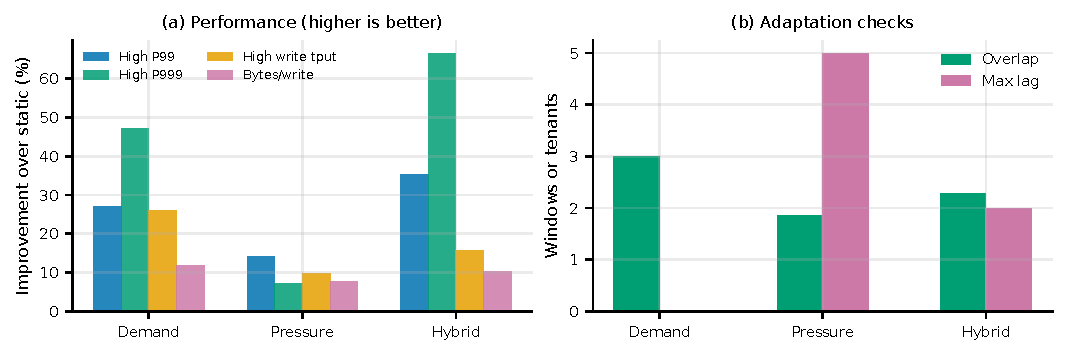
\includegraphics[width=0.88\textwidth]{fig4_score_ablation.pdf}
  \caption{Score-instance ablation. Demand mode gives strong high-pressure
  benefit while satisfying adaptation checks; pressure and hybrid instances
  improve some metrics but lag the moving high-pressure set.}
  \Description{Bar charts comparing demand, pressure, and hybrid score instances
  on normalized performance improvements, high-set overlap, and maximum lag.}
  \label{fig:score-ablation}
\end{figure*}

Is the runtime actuator really a maintenance I/O knob? The four-tenant
coverage microstudy in Section~\ref{sec:implementation} shows measured
limiter traffic rising monotonically with the configured budget and
compact-plus-flush output tracking it (coverage ratio 0.99--1.02) until the
workload's maintenance demand saturates near 7.3\,MB/s. This confirms the
continuous actuation path used by SAKI.

Is the result tied to one fragile score instance?
Section~\ref{sec:saki-design} treats the score
$s_i = 6.00\,D/1000 + 0.60\,G/1000 + 0.05\,T + 0.02\,B + 0.02\,P + 0.30\,L$
as an auditable reference instance, not an optimum. First, we replay the 35
post-warmup control decisions from the five continuous main online traces using
the previous-window observations that the controller saw. The replay exactly
reproduces the recorded online high-budget set in all 35 decisions. The demand
term alone also reproduces the reference top-four set in all 35 decisions;
anchor-dominant perturbations keep exact or near-exact top-four agreement,
while a pressure-only negative control matches only 10/35 decisions
(Table~\ref{tab:ranking-margin}). The reference score's top-four boundary
margin is positive in every replayed decision (mean 5.30, min 0.39), so the
main assignment is a property of a demand-aware score family rather than an
artifact of a single coefficient vector.

\begin{table}[!t]
  \centering
  \caption{Ranking-margin replay on the continuous main online traces
  (35 post-warmup decisions). Each score instance is recomputed from the
  previous-window observations; Jaccard compares its top-four set with the
  reference demand-mode top-four set.}
  \label{tab:ranking-margin}
  \small
  \setlength{\tabcolsep}{3.2pt}
  \begin{tabular}{lccc}
    \toprule
    Score instance & Exact & Jaccard & True overlap \\
    \midrule
    demand only & 35/35 & 1.00 [1.00,1.00] & 3.00/4 \\
    anchor $\times 0.5$ & 31/35 & 0.95 [0.33,1.00] & 2.86/4 \\
    anchor $\times 2$ & 35/35 & 1.00 [1.00,1.00] & 3.00/4 \\
    residual $\times 0.5$ & 35/35 & 1.00 [1.00,1.00] & 3.00/4 \\
    residual $\times 2$ & 31/35 & 0.95 [0.33,1.00] & 2.86/4 \\
    pressure-only & 10/35 & 0.61 [0.14,1.00] & 2.03/4 \\
    \bottomrule
  \end{tabular}
\end{table}

Second, we rerun nearby score instances on \runtimedrift by perturbing anchor
weight ($\times 0.5$, $\times 2$) and residual scale
($\times 0.5$, $\times 2$, $\times 0$, the last being anchor-only), with three
seeds each paired with the published paper-static trials a/b/c.
Table~\ref{tab:coefficient-ablation} shows that all five demand-aware
perturbations keep the headline direction, maintain overlap at
2.86--3.00/4, and keep max lag to 0--1 window. The \textsc{anchor-only} row,
where the residual scale is zero, is the runtime demand-only case: it confirms
the replay result that offered demand alone fixes the high-budget set, with
overlap 3.00/4 and zero lag. The residuals matter in the lower bound:
anchor-only high-throughput improvement drops as low as \(+12.6\%\), whereas
restoring half-strength residuals raises the minimum to \(+21.3\%\). This is consistent
with the division of labor in Section~\ref{sec:saki-design}: the demand anchor
tracks the active high-pressure set, while bounded pressure residuals appear to
stabilize near-boundary tenants whose maintenance state has not fully drained.
This is the empirical counterpart of Proposition~1: nearby demand-aware
instances keep the same placement behavior, whereas removing demand collapses
into the pressure-only case (Figure~\ref{fig:score-ablation}). Because the
ablation rows pair with only three static trials, row-to-row differences should
be read as consistency checks rather than tuning claims.

\begin{table*}[!t]
  \centering
  \caption{Score-family robustness around the demand-mode SAKI instance on
  \runtimedrift ($n{=}3$ per row, paired with paper-static a/b/c). Each row
  perturbs only the anchor or residual coefficients; all other settings are
  fixed. Cells show $\mathrm{mean}\,[\min,\max]$ percent of paired static;
  Top-4 Jaccard averages the post-warmup window-by-window high-set overlap
  against published SAKI decisions. The \textsuperscript{*} row reproduces
  the published $n{=}5$ main continuous result; its static pairing covers all
  five trials, not the three used by the ablation rows.}
  \label{tab:coefficient-ablation}
  \small
  \setlength{\tabcolsep}{4pt}
  \begin{tabular}{lccccc}
    \toprule
    Perturbation & High P99 & High tput & Overlap & Max lag & Top-4 Jaccard \\
    \midrule
    anchor $\times 0.5$ (3.00)        & -30.3\% [-38.1,-23.6] & +22.4\% [+18.9,+27.1] & 2.90/4 & 1 & 0.94 [0.88,1.00] \\
    anchor $\times 2$ (12.00)         & -27.5\% [-42.4,-18.2] & +23.7\% [+22.2,+26.2] & 3.00/4 & 0 & 1.00 [1.00,1.00] \\
    residual $\times 0.5$             & -30.0\% [-39.8,-16.7] & +24.3\% [+21.3,+28.2] & 3.00/4 & 0 & 1.00 [1.00,1.00] \\
    residual $\times 2$               & -35.8\% [-49.6,-25.7] & +25.0\% [+20.9,+27.1] & 2.86/4 & 1 & 0.94 [0.89,1.00] \\
    anchor only (residual$=0$)        & -31.9\% [-40.2,-26.2] & +21.5\% [+12.6,+26.0] & 3.00/4 & 0 & 1.00 [1.00,1.00] \\
    \midrule
    fixed SAKI (n=5, paper main)\textsuperscript{*} & -27.0\% & +26.1\% & 3.00/4 & 0 & 1.00 (self) \\
    \bottomrule
  \end{tabular}
\end{table*}

Finally, would a lower-layer control point be equivalent?
On the aligned epoch workload, online cgroup-v2 control improves high-pressure
throughput by 12.5\% relative to equal cgroup throttling, but the P99 CI
crosses zero (-4.4\%) and compaction bytes increase by 3.1\%. An oracle cgroup
assignment can express priority when the high-pressure set is known (P99
-9.1\%, throughput +15.4\%), so the layer is useful as an enforcement
envelope. It does not provide the LSM-aware budget-placement signal that SAKI
uses.

\subsection{Controlled Coverage Around the Anchor Workloads}
\label{sec:workload-matrix}

The next experiments test local coverage around the controlled anchor
workloads while preserving the same-budget contract. The epoch sensitivity
sweep changes drift speed and high-write pressure around \epochdrift. These
rows are local coverage checks: the promotion rule keeps capacity-boundary and
failed-tenant cases from obscuring the comparison, while the headline claim
rests on the repeated anchors above. All promoted points move in the headline
direction: high-pressure P99 improves by 6.9--12.9\%, high-pressure throughput
improves by at least 33.0\%, and compaction bytes fall by 17.6--21.3\%. The
faster-drift point remains CI-strict on high-pressure benefit (P99 -6.9\%,
throughput +33.9\%) with an aggregate-throughput cost (-5.0\%), matching the
expected responsiveness limit of a previous-window controller.

The continuous workload matrix changes one axis at a time around
\runtimedrift: 4\,KB values, tripled point-read QPS, faster drift at
1.5 tenants/window, and an 8-tenant cluster with two high-pressure tenants.
All four variants were promoted to five trials and retain the headline
direction: high-pressure P99 improves in every row and high-pressure
throughput improves by 20.1--30.4\%
(Table~\ref{tab:evaluation-workload-matrix}). Three rows are CI-strict wins
on both primary high-pressure metrics; \readthreex remains CI-strict on high
throughput, but its P99 confidence interval crosses zero. The matrix also
names the trade-off rather than hiding it: \valuefourk's P999 mean is negative
but not statistically separated from static, reflecting sparse
heavy-compaction bursts under a conserved rate-limit ceiling rather than a P999
regression. \readthreex is a point-read-QPS perturbation, not a scan-heavy or
read-dominant SLO result.

\begin{table*}[!t]
  \centering
  \caption{Local workload matrix, five trials per variant, online vs.\ static
  (percent changes, 95\% CI half-widths in pp).  Zero failed tenants in all
  runs.}
  \label{tab:evaluation-workload-matrix}
  \small
  \setlength{\tabcolsep}{2.8pt}
  \renewcommand{\arraystretch}{1.08}
  \begin{tabular}{lcccccr}
    \toprule
    Variant & High P99 & High P999 & High tput & Total tput & Bytes/write & Overlap \\
    \midrule
    \valuefourk   & -28.6\%$\pm$16.2 & -7.1\%$\pm$20.6  & +20.1\%$\pm$4.7  & +0.6\%$\pm$1.5  & -9.0\%$\pm$3.0  & 3.00/4 \\
    \readthreex   & -15.4\%$\pm$17.5 & -38.4\%$\pm$27.6 & +30.4\%$\pm$7.6  & -0.2\%$\pm$4.0  & -10.2\%$\pm$5.8 & 3.00/4 \\
    \fastdrift    & -17.6\%$\pm$10.1 & -1.1\%$\pm$46.6  & +20.5\%$\pm$10.3 & +4.4\%$\pm$3.4  & -3.3\%$\pm$4.4  & 2.57/4 \\
    \tenantseight & -42.2\%$\pm$12.7 & -52.6\%$\pm$16.9 & +28.7\%$\pm$5.8  & +7.0\%$\pm$1.9  & -11.3\%$\pm$3.4 & 1.57/2 \\
    \bottomrule
  \end{tabular}
\end{table*}

The window length is also a mechanism setting, not a tuned constant.
Table~\ref{tab:evaluation-window-length} repeats the continuous anchor at
10, 20, and 40 seconds with three seed pairs each, holding duration, offered
load, drift distance, and the 96\,MB/s aggregate budget fixed. The 20-second
anchor is the only point with a CI-strict high-P99 win (-26.9\%); 10 seconds
keeps high throughput positive but makes both P99 and throughput noisy and
raises LOW P99, while 40 seconds lowers overlap to 2.00/4 and leaves
adaptation lag unbounded in all three seeds. This supports using 20 seconds as
a mechanism-isolation anchor and treats the other two points as responsiveness
boundaries.

\begin{table}[!t]
  \centering
  \caption{Window-length sensitivity around the continuous anchor (three
  seed pairs per row, online vs.\ static; CI half-widths in pp).}
  \label{tab:evaluation-window-length}
  \small
  \setlength{\tabcolsep}{3.0pt}
  \begin{tabular}{lcccc}
    \toprule
    Window & High P99 & High tput & Overlap & LOW P99 \\
    \midrule
    10\,s & +6.8\%$\pm$39.2  & +23.4\%$\pm$58.1 & 3.47/4 & +110.5\%$\pm$367.8 \\
    20\,s & -26.9\%$\pm$14.0 & +16.1\%$\pm$8.7  & 3.00/4 & +24.6\%$\pm$63.6 \\
    40\,s & -14.4\%$\pm$44.8 & +14.5\%$\pm$19.8 & 2.00/4 & -36.3\%$\pm$84.2 \\
    \bottomrule
  \end{tabular}
\end{table}

\subsection{Collateral Cost and Liveness}

SAKI is a targeted reallocation policy, not a Pareto-improvement claim.
Tier-level accounting makes the redistribution explicit. In the continuous
aggregate, HIGH tenants receive P99 -27.0\%, P999 -47.1\%, and write
throughput +26.1\%; LOW tenants absorb P99 +1.4\%, P999 +2.6\%, and write
throughput -3.0\%. The epoch-level pattern is similar: HIGH throughput rises
by 38.1\%, while MID and LOW throughput change by -9.1\% and -1.2\%. Total
throughput remains close to static in both harnesses, so the benefit is a
budget-placement trade-off rather than added capacity.

\begin{figure*}[!t]
  \centering
  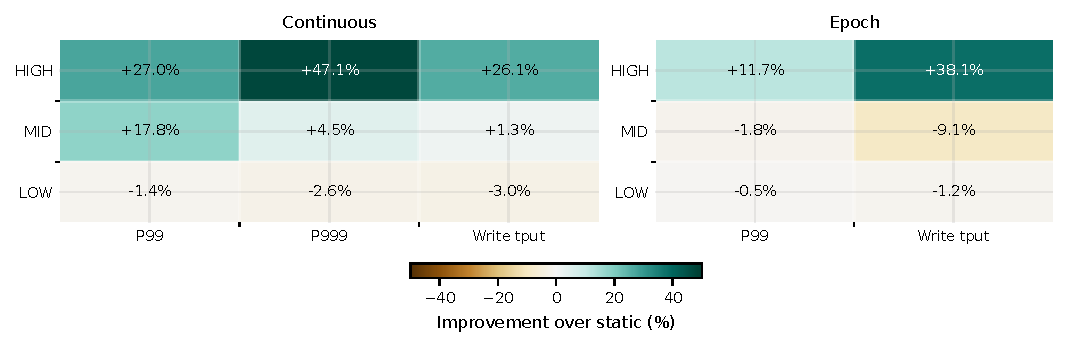
\includegraphics[width=0.82\textwidth]{fig8_collateral_summary.pdf}
  \caption{Tier-wise benefit and collateral cost. Cells report SAKI's
  improvement over static (positive is better), showing the intended
  high-pressure benefit and the measured redistribution cost to lower tiers.}
  \Description{Two-panel matrix for continuous and epoch runs, showing P99,
  P999, and throughput changes by high, mid, and low tiers.}
  \label{fig:collateral-summary}
\end{figure*}

Read-side and CPU measurements show that the bytes/write improvement does not
hide higher compaction CPU per completed write: CPU/write falls by 12.8\%
overall. The tier values are -1.6\% for HIGH, -8.0\% for MID, and -33.5\%
for LOW. Read-side effects are bounded in this read-light workload (overall
read P99 +7.0\%, read P999 -10.6\%, read throughput +0.5\%), but they are
collateral accounting rather than evidence for read-dominant SLOs. A separate
360-second continuous run with 16 drift events reports high P99 $-13.9\%$,
high P999 $-19.6\%$, high write throughput $+11.6\%$, bytes/write $-3.4\%$,
overlap $3.00/4$, max lag $1$~window, and zero tenant failures---a liveness
and tracking sanity check at the longer horizon.

\subsection{Trace Qualification Boundary}
\label{sec:public-trace}

The controlled experiments above establish the fixed-budget placement
mechanism. Public traces become meaningful controller-validation workloads
when they preserve tenant identity and drift, expose actuatable supply under
the fixed budget, and create enough RocksDB maintenance stress to exercise
compaction-budget placement. We audited two public trace families under the
same 11/7/3\,MB/s, 112\,MB/s budget contract and use them to identify which of
those conditions are missing.

Meta CacheLib \texttt{kvcache/202401}~\cite{cachelib_trace} is useful as a
trace-shaped replay and tracking smoke, but it records cache-front-end
requests rather than RocksDB compaction events. Five selected drifting
16-tenant segments completed with zero failed tenants and preserved drift, yet
the replay failed the engine-stress gate: offered writes were 110--143\,MB/s,
completed logical writes were only 6.7--7.3\,MB/s, compaction output plateaued
near 29--31\,MB/s, and no segment entered the stress-pass subset. Meta
Tectonic/Baleen storage 0.1\%~\cite{baleen_fast24} exposes the complementary
condition. Aggregate scaled write supply initially looked sufficient, but most
windows have only one to three active write tenants. Under the static all-mid
policy, the actuatable supply \(\sum_i \min(7,\mathrm{traceWrite}_i)\) is far
below the aggregate trace rate; across 146 independent candidates, zero have
six or more windows above 70\,MB/s or mean static-actuatable supply above
70\,MB/s. These audits are therefore trace-qualification results rather than
controller comparisons.

\section{Discussion and Limitations}

\subsection{Applicability Conditions}
\label{sec:discussion-drift}

SAKI applies when co-located RocksDB instances share a fixed background budget,
write pressure drifts across tenants at window time scales, and the host can
observe tenant-local demand and maintenance symptoms. The repeated epoch runs
establish the main placement effect, the continuous runs show that it survives
runtime rate-limiter actuation, and the mechanism checks rule out stale skew,
tenant-local autotuning, pressure-only tracking, lower-layer throttling, and a
non-maintenance actuation path. Ranking-margin replay and perturbation runs
further show that the main continuous high-budget assignment is fixed by a
demand-aware score family rather than by one isolated coefficient vector.
Together, these results support the systems claim that a host-level
rank-and-assign controller can place an existing compaction/I/O budget better
than equal sharing.

The bounded-drift condition matters. SAKI relies on previous-window
observations remaining relevant to the next window. The main continuous
workload moves the high-pressure set by one tenant per 20-second window, and
\fastdrift pushes this to 1.5 tenants/window while retaining
CI-strict high-pressure benefit with overlap 2.57/4. Abrupt reversals,
sub-window bursts, and within-window phase changes may outrun the controller.
The 20-second window, 4/8/4 tier split, and concrete budget levels are
mechanism-isolation settings. In the continuous anchor, a 10/20/40-second
window sweep keeps the 96\,MB/s budget fixed and brackets the trade-off:
10 seconds improves assignment frequency but makes high-P99 and LOW collateral
noisier, whereas 40 seconds reduces overlap and leaves adaptation unbounded in
all three seeds. The conservation rule in Section~\ref{sec:saki-design}
supports other tier counts, budget spreads, or a continuous allocator.

\subsection{Deployment Assumptions}

The continuous harness changes background rate limits through \ratecall. The
measured rate-limiter coverage microstudy shows this knob shapes
flush/compaction I/O in our configuration, so foreground latency and
throughput changes arise indirectly from maintenance service rather than
direct foreground throttling. RocksDB's built-in auto-tuned rate limiter
remains useful local machinery, but it adapts within per-tenant ceilings;
SAKI supplies the host-level loop that moves unused budget across tenants. A
natural deployment variant is to let SAKI choose tenant ceilings while RocksDB
autotuning adapts inside each ceiling; we did not evaluate that combined
policy.

A production deployment would need tenant inventory, periodic RocksDB
statistics, a conserved host budget, and per-tenant runtime actuation. The
offered-demand signal should be measured near admission, such as at a client
proxy, RPC ingress path, tenant queue, or write-admission counter, before
upstream backpressure, drops, or retries hide true pressure. Operators would
likely add smoothing, hysteresis, cooldowns, minimum dwell times, and SLO-aware
floors around the simple rank-and-assign rule. If metrics or tenant inventory are
missing, the safe operational choice is to retain the last valid assignment or
fall back to all-mid sharing, preserving the aggregate budget before
re-enabling reallocation. The reference score should be treated as a
demand-aware instance of the framework, not as a portable constant vector:
deployments with different admission signals or maintenance dynamics should
renormalize terms while preserving budget conservation and demand observability.
Other LSM engines need analogous tenant-scoped maintenance signals and a
runtime maintenance-budget knob.

\subsection{Resource and Fairness Boundaries}

SAKI controls one resource dimension: background I/O budget placement. CPU,
cache, memory, device queueing, and per-level write amplification may become
the limiting resources in other deployments. A deployment can detect this
regime when rate-limiter traffic stops tracking flush/compaction output or
when CPU, cache, or device-queue metrics saturate while compaction debt remains
high. The continuous efficiency metric is therefore normalized bytes/write
because SAKI completes more foreground writes; a full maintenance-cost
decomposition is a separate multi-resource control problem.

The policy is also a targeted reallocation. Tier-wise reporting makes the
collateral cost explicit because shifting budget to high-pressure tenants can
cost lower-pressure tenants. In the main continuous aggregate, LOW tenants see
small write-tail and throughput costs while HIGH tenants improve substantially;
the 4\,KB-value workload leaves P999 not CI-separated from zero despite a
CI-strict P99 win.
These results motivate SLO-aware floors and fairness policy as deployment
layers around the same fixed-budget loop. The read-heavy variant raises
point-read QPS around the main harness; scan-heavy workloads, range-scan SLOs,
and read-dominant deployments require their own scoring and validation layer.

\subsection{Trace Validation Boundary}

The public-trace audits define the conditions required for meaningful
controller validation. CacheLib provides real cache-front-end request traces
and validates trace-shaped replay plumbing, but the selected segments create
too little RocksDB maintenance stress: completed logical writes were only
about 5--6\% of offered demand and compaction output plateaued near 30\,MB/s.
Baleen exposes a different issue: aggregate scaled write supply can look
adequate while too few tenants are active in each window to actuate the fixed
all-mid budget. Across 146 independent candidates, no segment had enough
static-actuatable supply to justify a second static smoke.

The next production-trace validation layer needs storage-engine traces with
tenant identity, drift, sustained write pressure, and actuatable supply under
the same fixed-budget contract. Non-leveled compaction styles, longer
deployments, and joint multi-resource control are natural extensions after
that trace condition is met.

\section{Related Work}

\paragraph{LSM compaction and tuning.}
The original LSM-tree design buffers updates and later merges them into
disk-resident sorted components~\cite{oneil1996lsm}. The survey by Luo and
Carey describes the resulting design space~\cite{luo2020lsmsurvey}, and
Sarkar et al.\ formalize compaction triggers, layout, granularity, and data
movement as design primitives~\cite{sarkar2021lsmspace}. Monkey and
Dostoevsky optimize Bloom-filter memory, merge policy, and space-time
tradeoffs~\cite{dayan2017monkey,dayan2018dostoevsky}; WiscKey and PebblesDB
change value placement or merge structure~\cite{lu2016wisckey,raju2017pebblesdb}.
bLSM, TRIAD, and Accordion improve write smoothing, logging, and memory
organization~\cite{sears2012blsm,balmau2017triad,bortnikov2018accordion}.
SILK schedules internal LSM I/O to reduce latency spikes, while ADOC, vLSM, and
ArceKV tune dataflow, LSM shape, or compaction thresholds for a single engine
or workload~\cite{balmau2019silk,yu2023adoc,xanthakis2024vlsm,liu2026arcekv}.
Dremel adaptively tunes \rocksdb parameters with an online bandit on a single
instance~\cite{zhao2022dremel}, and Dong et al.'s \rocksdb retrospective at
Meta tracks how amplification priorities shifted with hardware and workload,
still inside one engine~\cite{dong2021rocksdbevolution}. SAKI is orthogonal:
it leaves each engine's compaction policy and parameters unchanged, treats
these single-engine contributions as the inner control loop, and asks how a
fixed host budget should be divided across co-located instances as demand
drifts. The two control layers can be combined.

\paragraph{Multi-tenant storage control.}
Argon, PARDA, mClock, Pisces, Cake, and IOFlow allocate or route storage
service across shared servers, hypervisors, and software-defined storage
planes~\cite{wachs2007argon,gulati2009parda,gulati2010mclock,shue2012pisces,
wang2012cake,thereska2013ioflow}. Linux cgroups and IOCost provide lower-layer
block-I/O weighting~\cite{linux_cgroup_v2,heo2022iocost}, and Gimbal extends
the line to SmartNIC JBOFs that schedule co-tenant NVMe traffic on the
storage data path~\cite{min2021gimbal}. These systems enforce fairness or
SLOs over I/O streams but do not observe LSM debt signals or choose which
\rocksdb instance receives background compaction service. SAKI uses those
engine-level signals and treats kernel or network-side I/O control as a
companion enforcement layer rather than the placement mechanism itself.

\paragraph{Multi-tenant LSM deployments.}
Recent KV-store work moves isolation closer to the storage engine. FlexEngine
uses admission control for multi-tenant serverless LSM deployments, Iso-KVSSD
and ZenFS+ use device namespace or zoned-placement mechanisms for isolation,
and Delta Fair Sharing proposes in-engine multi-tenant fairness for
RocksDB~\cite{wang2026flexengine,min2021isokvssd,oh2023zenfs,
griggs2026deltafairsharing}. CaaS-LSM and DFlush move compaction or flush work
into disaggregated or DPU-assisted settings~\cite{yu2024caaslsm,ding2025dflush}.
SAKI instead targets the common deployment where tenants are separate,
unmodified RocksDB instances on one host and the available background budget is
fixed.

\paragraph{RocksDB controls.}
RocksDB exposes per-instance options, statistics, event listeners, and rate
limiting~\cite{rocksdb,rocksdb_ratelimiter}. The auto-tuned rate limiter solves
local adaptation within a ceiling; SAKI supplies the host-level rank-and-assign
loop that places budgets across instances under a conserved aggregate budget.
Public CacheLib and Baleen traces inform our trace-qualification audits, but
cache admission, prefetching, or request-trace replay are separate from the
fixed-budget RocksDB compaction-placement problem~\cite{cachelib_trace,
baleen_fast24}. SAKI reallocates a conserved host budget across separate
instances without changing the engine.

\section{Conclusion}

SAKI addresses multi-tenant \rocksdb compaction-debt mismatch with an external
conserved rank-and-assign controller that reallocates per-tenant background
budgets from previous-window observations while preserving the aggregate host
budget. A demand-observability model explains why demand-aware ranking keys
track bounded drift and why pressure-only ranking can chase stale debt.
Repeated epoch and continuous runs show
high-pressure write-tail and throughput gains; stronger baselines, ranking-key
ablations, ranking-margin replay, cgroup-v2, and rate-limiter coverage checks
tie those gains to host-level placement of a real maintenance-I/O knob.
Workload variants, collateral accounting, and trace qualification define the
current evidence boundary. For bounded write-heavy drift under fixed shared
maintenance budgets, SAKI shows that shared compaction budgeting is not merely
a configuration detail but a host-level control point.


\bibliographystyle{ACM-Reference-Format}
\bibliography{saki_refs}

\end{document}
